\documentclass[14pt]{beamer}
\usepackage[english,russian]{babel}
\usepackage[utf8]{inputenc}
\usepackage{listings}
\usepackage{tikz}
\usepackage{graphicx}
\usetikzlibrary{arrows,decorations.pathmorphing,backgrounds,fit,positioning,shapes.symbols,chains}

\setbeamersize{text margin left=6mm, text margin right=6mm}

\linespread{1.2}

% Стиль презентации
\usetheme{Amsterdam}

%gets rid of bottom navigation bars
\setbeamertemplate{footline}[page number]{}

%gets rid of navigation symbols
\setbeamertemplate{navigation symbols}{}

\beamertemplatenavigationsymbolsempty

\begin{document}
\title{Синтез объектно-ориентированных интерфейсов из декларативных описаний форматов данных и библиотек}
\author{Игнатов С.С., группа 6057/1}
% \institute{Санкт-Петербургский государственный политехнический университет \\
% Физико-механический факультет \\
% Кафедра прикладной математики}
\date{Санкт-Петербург, 2012}

\frame{\linespread{1}\titlepage}

% \frame{\frametitle{Содержание}\tableofcontents[currentsection]}

\begin{frame}\frametitle{Внешние источники данных}
\linespread{1}

\begin{tikzpicture}
[node distance = 1cm, auto,
% STYLES
every node/.style={node distance=2cm},
% The comment style is used to describe the characteristics of each force
comment/.style={rectangle, inner sep=5pt, text width=2.5cm, node distance=0.25cm, font=\scriptsize\sffamily},
% The force style is used to draw the forces' name
force/.style={rectangle, draw, fill=blue!5, inner sep=5pt, text width=2.85cm, text badly centered, minimum height=1.2cm, font=\bfseries\footnotesize\sffamily}]

% Draw forces
\node [force] (rivalry) {Программа};
\node [force, above of=rivalry] (substitutes) {XML};
% \node [force, text width=3cm, dashed, left=1cm of substitutes] (state) {Public policies};
\node [force, left=1cm of rivalry] (suppliers) {База данных};
\node [force, right=1cm of rivalry] (users) {WSDL};
\node [force, below of=rivalry] (entrants) {Библиотека на C};

% RIVALRY
\node [comment, below=0.25 of rivalry] (comment-rivalry) {};
% SUPPLIERS
\node [comment, below=0.25cm of suppliers] {};
% SUBSTITUTES
\node [comment, right=0.25 of substitutes] {};
% USERS
\node [comment, below=0.25 of users] {};
% NEW ENTRANTS
\node [comment, right=0.25 of entrants] {};
% PUBLIC POLICIES
% \node [comment, text width=3cm, below=0.25 of state] {};

% Draw the links between forces
\path[-stealth, thick]
    (rivalry) edge (substitutes)
    (rivalry) edge (suppliers)
    (rivalry) edge (users)
    % (rivalry) edge (state)
    (rivalry) edge (entrants);

\end{tikzpicture}
    \center{\small{\textbf{Проблема:} корректно ли использование внешних ресурсов?}}
\end{frame}

\begin{frame}\frametitle{Постановка задачи}

    \textbf{Цель:} гарантировать корректность работы с внешними источниками.

    \textbf{Задачи:}
    \begin{itemize}
        \item[---] {<<Встроить>>} в язык программирования
        \item[---] Реализовать расширения компилятора для работы с XML и C
        \item[---] Сравнить полученные результаты с аналогами
        \item[---] Получить опыт разработки подобных механизмов
    \end{itemize}
    % Разработать механизм работы с внешними источниками данных.

    % Важные свойства:
    % \begin{itemize}
    %     \item[---] Статическая типизация
    %     \item[---] Синхронизация с интерфейсом
    %     \item[---] Удобство использования
    %     \item[---] Поддержка в среде разработки
    % \end{itemize}
    % Создать реализации для работы с XML и языком C.

\end{frame}

\begin{frame}\frametitle{Обзор существующих решений} % TODO
    \begin{itemize}
        \item[---] Поставщики типов (type providers) в языке F\#
        \item[---] Загрузчики типов (type loaders) в языке Gosu
    \end{itemize}
\end{frame}

\begin{frame}\frametitle{Язык программирования Kotlin}
    \begin{itemize}
        \item[---] Объектно-ориентированный
        \item[---] Статически типизированный
        \item[---] Компилируется в байт-код для JVM
        \item[---] Общего назначения
    \end{itemize}
\end{frame}

\begin{frame}\frametitle{Архитектура компилятора}
\linespread{0.9}
\begin{small}
    Фазы компиляции:
    \begin{itemize}
        \item[---] Лексический анализ
        \item[---] Синтаксический анализ
        \item[---] Построение внутреннего представления
        \item[---] Анализ типов
        \item[---] \textbf{Трансформация внутреннего представления программы}
        \item[---] \textbf{Повторный анализ типов}
        \item[---] Генерация байт-кода
    \end{itemize}
\end{small}
\linespread{1.2}
\end{frame}

\begin{frame}\frametitle{Пример использования XML}
\begin{center}
    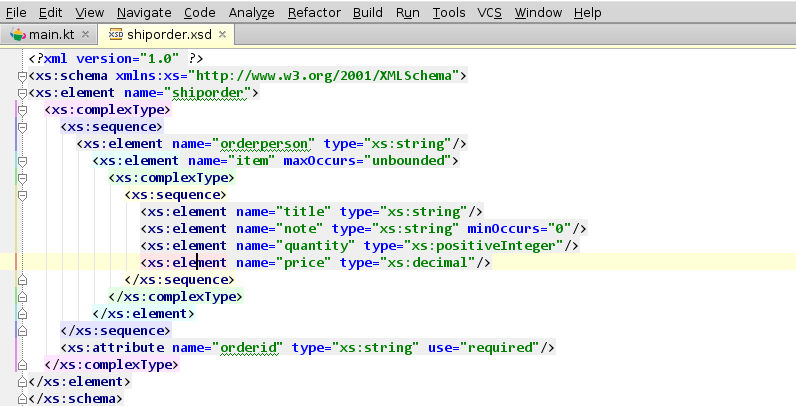
\includegraphics[height=4.5cm,width=8.48cm]{shiporder}

    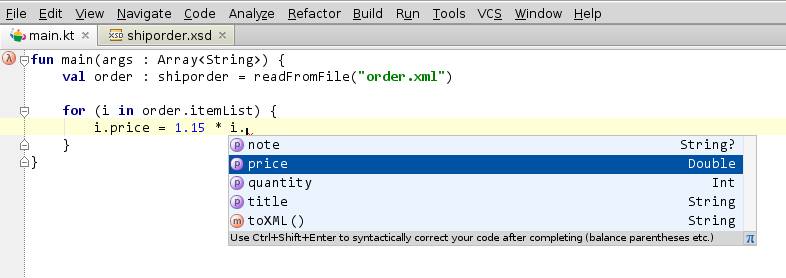
\includegraphics[height=3cm,width=8.48cm]{completion}
\end{center}
\end{frame}

\begin{frame}\frametitle{Пример использования C}
\end{frame}

\begin{frame}\frametitle{Основные результаты}
    Качественные улучшения:
    \begin{itemize}
        \item[---] Согласованность с внешними интерфейсами
        \item[---] Упрощение рабочего процесса программиста
        \item[---] Отсутствие сгенерированных артефактов в системе контроля версий
    \end{itemize}
\end{frame}

\begin{frame}\frametitle{Количественные улучшения}
    \begin{itemize}
        \item[---] Лаконичный код:
            \begin{itemize}
                \item[---] сопоставим с Gosu
                \item[---] в 2--3 раза меньше, чем Java
            \end{itemize}
        \item[---] Уменьшение размера бинарной сборки за счет удаления типовой информации
    \end{itemize}
\end{frame}

\begin{frame}\frametitle{Заключение}
Реализованы механизмы загрузки типов для XML и языка C.

\textbf{Результаты:}
    \begin{itemize}
        \item[---] Статические гарантии корректности
        \item[---] Уменьшение объема исходного кода
        \item[---] Упрощение рабочего процесса
    \end{itemize}
\end{frame}

\end{document}

% listing example
% \frame[containsverbatim]{
% \frametitle{Source code}

% \begin{lstlisting}[language=C]
% int main() {
%     printf("Hello World!");
%     return 0;
% }
% \end{lstlisting}
% }
